\begin{figure}[htbp]
\centering
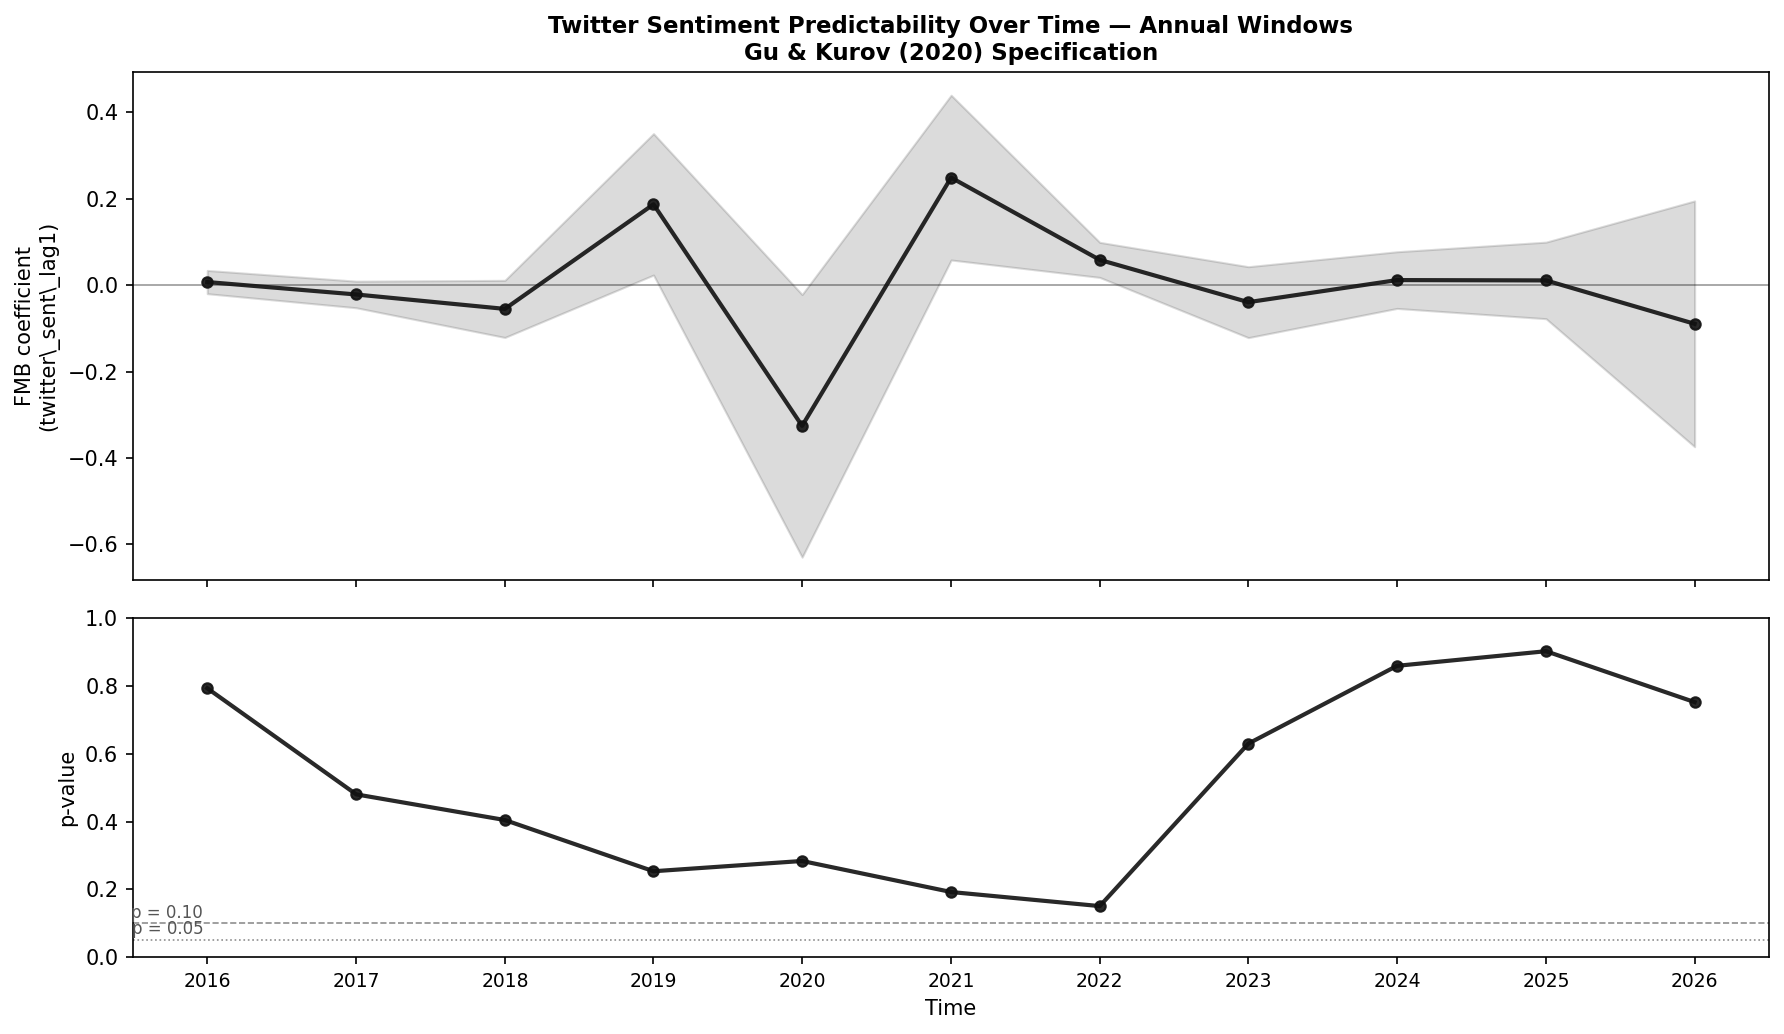
\includegraphics[width=\linewidth]{figures/gk_temporal_annual.png}
\caption{Twitter Sentiment Predictability Over Time --- Gu \& Kurov (2020) Specification (Annual windows). Top panel: Fama-MacBeth coefficient on \texttt{twitter\_sent\_lag1} with $\pm$1 SE band. Bottom panel: associated $p$-value; dashed lines at $p = 0.10$ and $p = 0.05$. Annual windows (one observation per calendar year). Bandwidth = 5 lags; minimum cross-section $N = 30$.}
\label{fig:gk_temporal_annual}
\end{figure}

\begin{figure}[htbp]
\centering
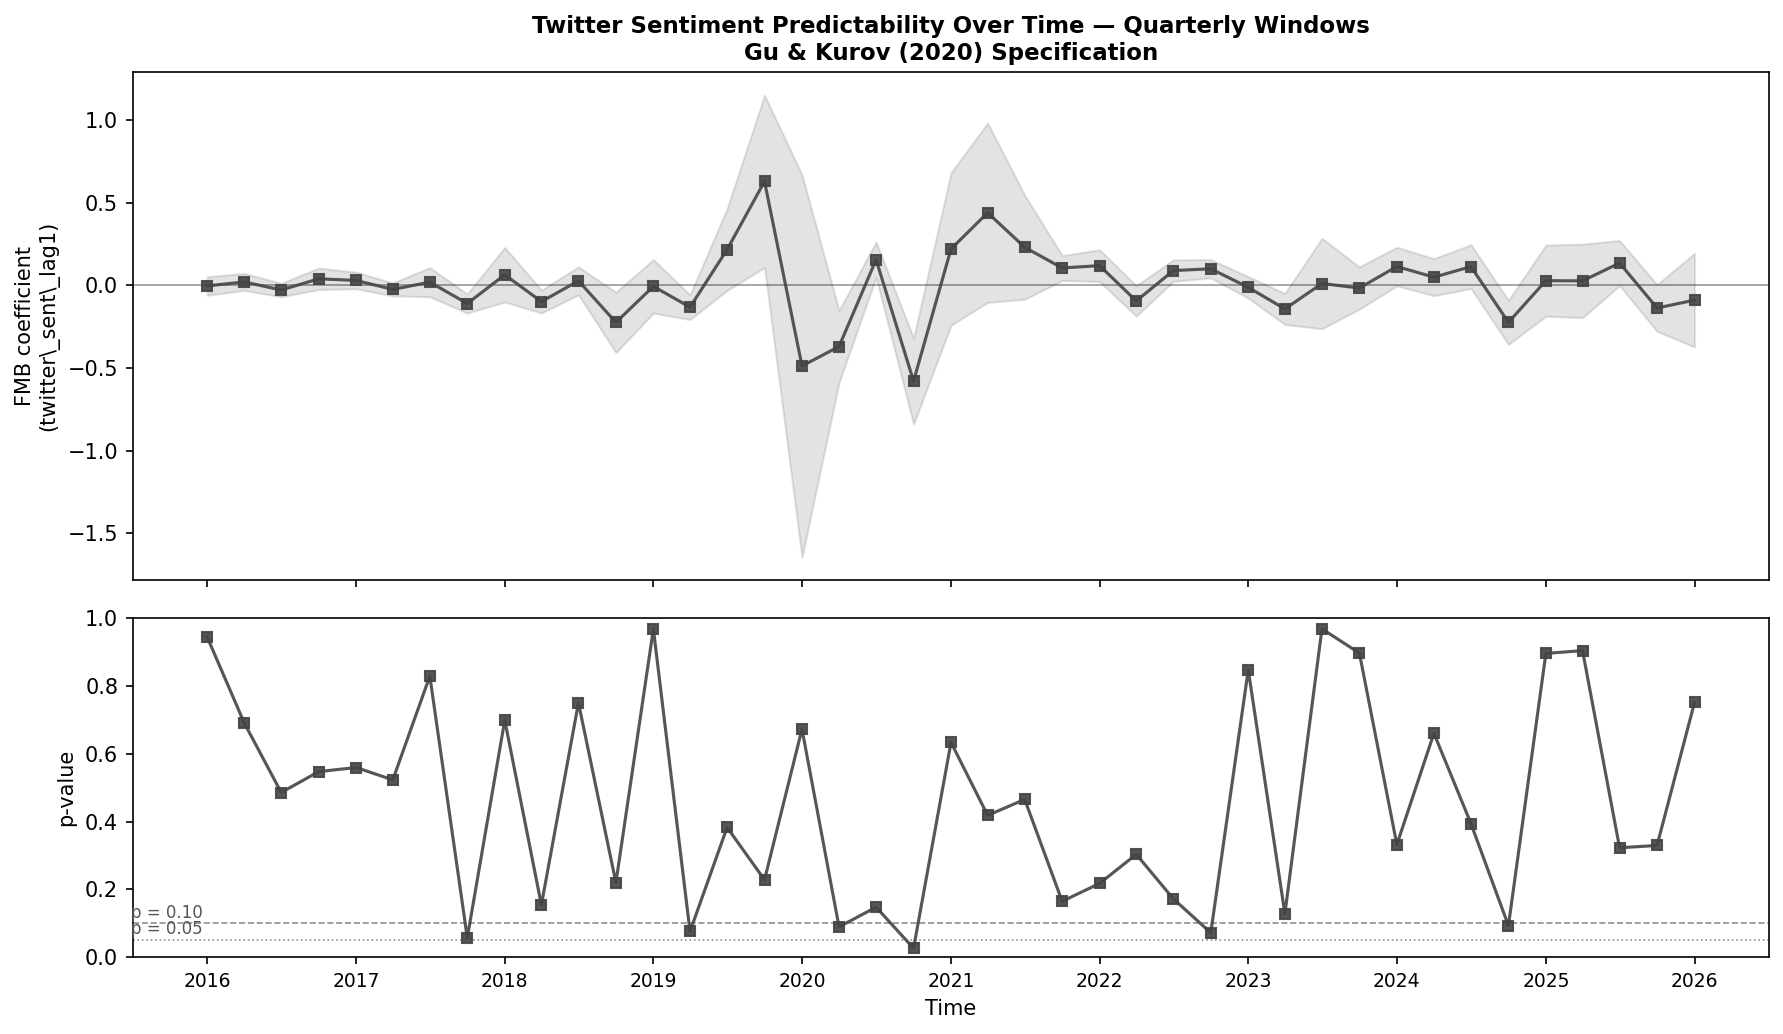
\includegraphics[width=\linewidth]{figures/gk_temporal_quarterly.png}
\caption{Twitter Sentiment Predictability Over Time --- Gu \& Kurov (2020) Specification (Quarterly windows). Top panel: Fama-MacBeth coefficient on \texttt{twitter\_sent\_lag1} with $\pm$1 SE band. Bottom panel: associated $p$-value; dashed lines at $p = 0.10$ and $p = 0.05$. Quarterly windows. Bandwidth = 4 lags; minimum cross-section $N = 20$.}
\label{fig:gk_temporal_quarterly}
\end{figure}

\begin{figure}[htbp]
\centering
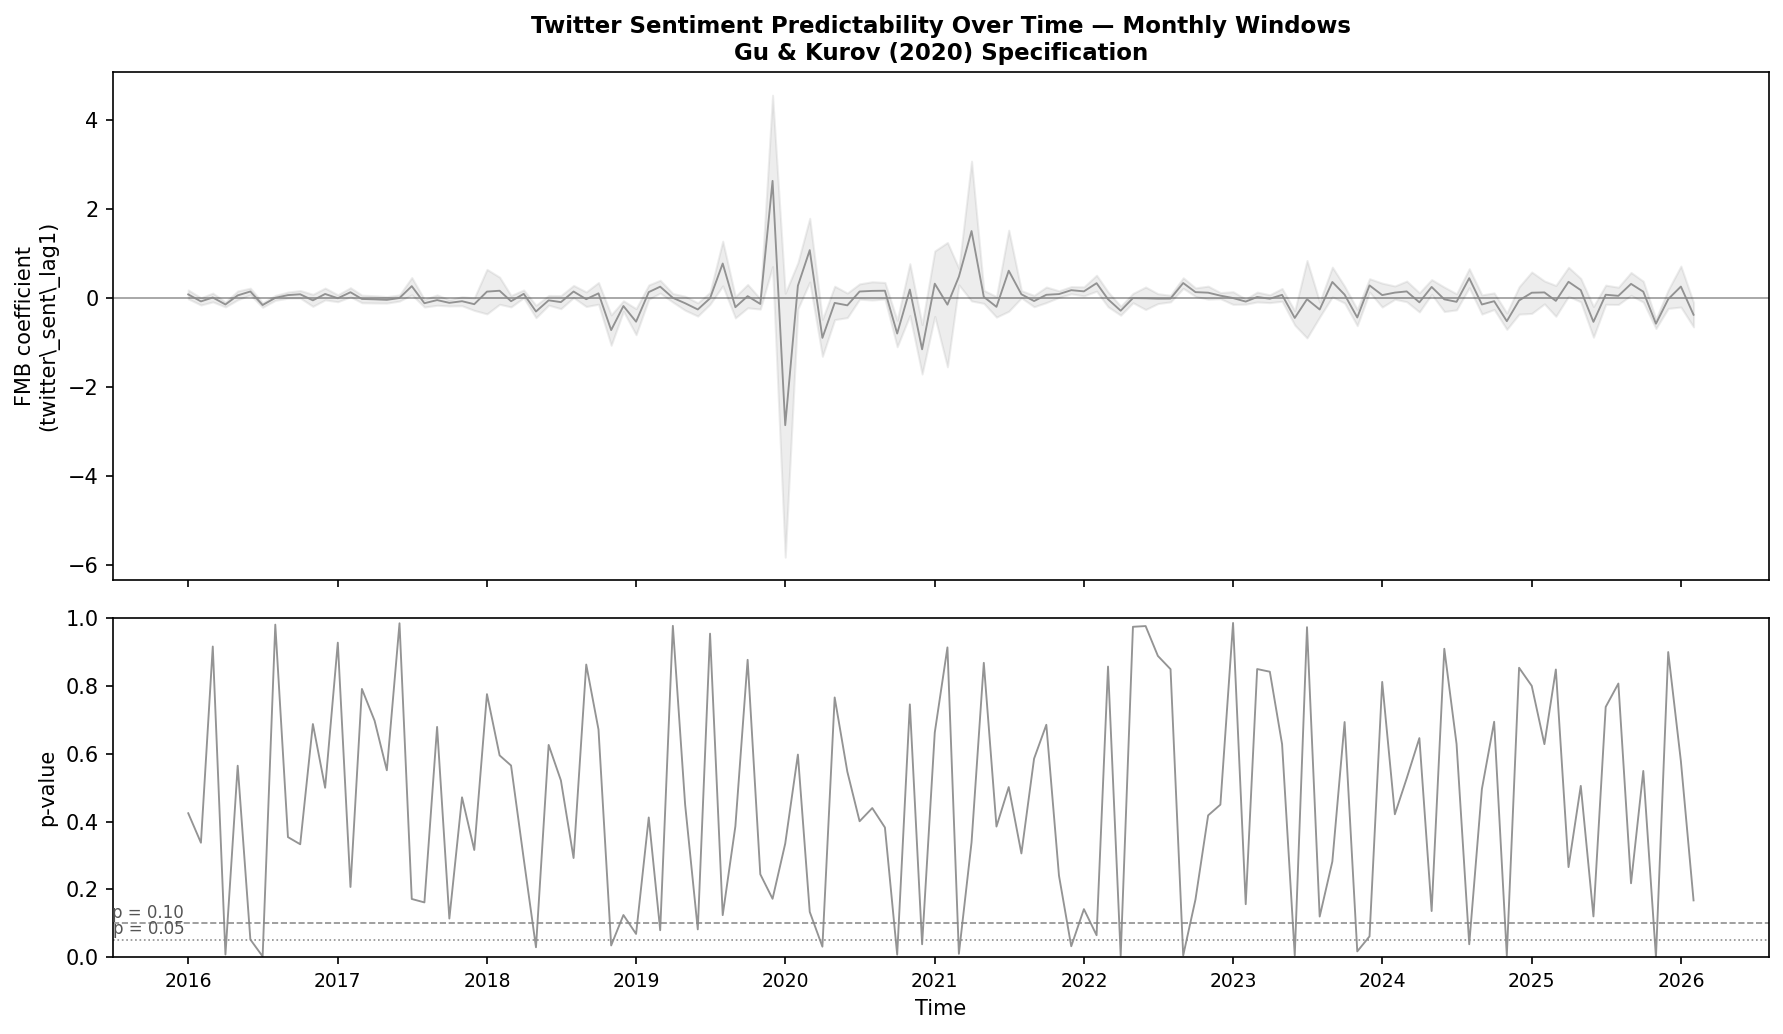
\includegraphics[width=\linewidth]{figures/gk_temporal_monthly.png}
\caption{Twitter Sentiment Predictability Over Time --- Gu \& Kurov (2020) Specification (Monthly windows). Top panel: Fama-MacBeth coefficient on \texttt{twitter\_sent\_lag1} with $\pm$1 SE band. Bottom panel: associated $p$-value; dashed lines at $p = 0.10$ and $p = 0.05$. Monthly windows. Bandwidth = 3 lags; minimum cross-section $N = 15$.}
\label{fig:gk_temporal_monthly}
\end{figure}